Измерение расстояния методом \textit{Time of Flight} ограничено такими факторами, как синхронизация во времени, шумы, погрешности выборки и эффект многолучевого распространения. Этот раздел обобщает информацию о каждой возможной причине.

\subsubsection{Синхронизация во времени}

\textit{Time of Flight} системе необходимо измерить время между отправкой и принятием сигнала, используя общий отсчёт времени. В простейшем случае, устройство Б определяет удалённость от устройства А измеряя время прибытия сигнала от устройства А. Если "часы" синхронизированы не идеально (рисунок~\ref{fig:sync}), т. е. начало отсчёта t = 0 устройства Б содержит некоторое смещение относительно нуля устройства А, это добавляет дополнительную ошибку в измерение. Необходимая дискретизация синхронизации времени (1 нс = 30 см) зачастую слишком точная для многих систем~\cite{tof:lowcost}.

\begin{figure}[ht]
    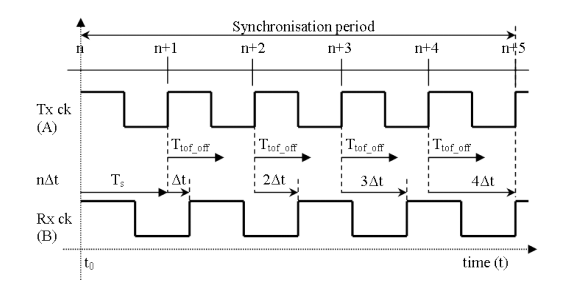
\includegraphics[width=.8\linewidth]{Figures/sync.png}
    \caption{Рассинхронизация частот двух тактовых генераторов}
    \label{fig:sync}
\end{figure}

Рассинхронизацию часов можно устранить при помощи метода <<Two Way Time Transfer>>, про который будет рассказано в главе~\ref{sec:mitigation} <<\nameref{sec:mitigation}>>.

\subsubsection{Шум}

Точность измерения расстояния в идеальном случае ограничего лишь белым шумом --- отношением <<энергия/шум>>, $E_S/N_0$ на приёмнике и используемой шириной частоты (bandwidth), $B$. Измерение дальности --- вопрос, изучаемый в контексте радаров, и неравенство Крамера-Рао обеспечивает нахождение нижней границы дисперсии оценки диапазона белого шума. Для односторонней системы нахождения расстояния используя IEEE 802.15.4 модуляцию, неравенство Крамера-Рао выглядит так (формула~\eqref{eq:crb}):

\begin{equation}
    \label{eq:crb}
    \sigma_r^2 >= \frac{c^2}{\frac{4 \pi^2 B^2 E_S}{N_0}},
\end{equation}

где $\sigma_r^2$ --- дисперсия оценки диапазона,
$c$ --- скорость света,
и $B$ --- используемая ширина полосы сигнала в Герцах.

Отношением <<сигнал/шум>> здесь является (формула~\eqref{eq:snr}):

\begin{equation}
    \label{eq:snr}
    \frac{E_S}{N_0} = t_S B \cdot SNR,
\end{equation}

где $t_S$ --- длительность сигнала, на время которого ширина полосы занята.

В большинстве сигналов, ширина полосы и длительность завязаны таким образом, что $t_S B \approx 1$. Таким образом, соотношение $\frac{E_S}{N_0}$ приблизительно равно SNR (отношению <<сигнал/шум>>).

Сигналы с $t_S B > 1$ будут проявлять лучшее шумоподавление за счет более низкого соотношения <<сигнал/шум>>, и таких сигналы называются <<pulse-compressed waveforms>>.

%\subsubsection{Погрешности выборки}

%Здесь про выборку.

%\subsubsection{Multipath channel effect}

%Здесь про многолучевое распространение.
